\documentclass{article}

\usepackage[final]{corl_2023}

\usepackage{amsmath,amssymb}
\usepackage{graphicx}
\usepackage{booktabs}
\usepackage{xcolor}
\usepackage{multirow}

% Placeholder marker for numbers/text the team still has to fill in.
\newcommand{\todo}[1]{\textcolor{red}{[TODO: #1]}}
\newcommand{\R}{\mathbb{R}}
\newcommand{\bfF}{\mathbf{F}}

\title{Deep RL-based Control of a Quadrotor with a\\Double Pendulum Payload: Progress Report}

\author{
  Aashish Dhanani\\
  Robotics Institute\\
  Carnegie Mellon University\\
  \texttt{aashishd@andrew.cmu.edu} \\
  \And
  Percy Wu\\
  Robotics Institute\\
  Carnegie Mellon University\\
  \texttt{percyw@andrew.cmu.edu} \\
  \And
  Rian Borah\\
  Robotics Institute\\
  Carnegie Mellon University\\
  \texttt{rborah@andrew.cmu.edu} \\
  \AND
  Shayaan Shaikh\\
  Robotics Institute\\
  Carnegie Mellon University\\
  \texttt{shayaans@andrew.cmu.edu} \\
  \And
  Trevor Chartier\\
  Robotics Institute\\
  Carnegie Mellon University\\
  \texttt{tchartie@andrew.cmu.edu} \\
  \And
  Claude Opus 5.5 High\\
  Anthropic, PBC\\
}

\begin{document}
\maketitle

%===============================================================================
\begin{abstract}
We report progress on learning a controller that damps the oscillations of a
double-pendulum payload hanging from a quadrotor. We built planar and 3D MuJoCo
simulations of the system and a Gymnasium interface whose actions are collective
thrust and body rates. We also implemented the classical baselines from our
proposal: an LQR controller linearized about hover, and a payload-unaware
flatness-based tracking controller for both models. In the planar model, LQR
recovers from impulsive pushes up to the largest we tested, while the payload-unaware
controller holds position but leaves the payload swinging. The tracking controllers
follow circles, figure-eights and waypoint paths to within about 1\,cm RMS. Because
the pendulum hangs from single-axis bearings, the vehicle's effective pitch inertia
is about $11\times$ its roll inertia, and a controller tuned for the bare drone
becomes unstable in 3D. PPO training on the planar hover task is under way.
\end{abstract}

\keywords{Reinforcement Learning, Aerial Manipulation, Underactuated Systems}

%===============================================================================
\section{Introduction}
\label{sec:intro}

A quadrotor carrying a load on a chain of links is underactuated and strongly
nonlinear. The double-pendulum payload is chaotic at large swing angles, and the
linearized models used by classical controllers are only valid near hover with the
links hanging straight down. Our proposal is to learn a disturbance-recovery
controller with model-free deep RL (PPO~\citep{schulman2017ppo},
SAC~\citep{haarnoja2018sac}, TD3~\citep{fujimoto2018td3}), compare it against an LQR
controller and a payload-unaware quadrotor controller, and test sim-to-real transfer on
hardware. Model-based methods handle a single rigid or cable-suspended
load~\citep{sreenath2013geometric,palunko2012trajectory} but become much harder to
derive with a second link. RL has controlled quadrotors from aggressive initial
conditions~\citep{hwangbo2017control,kaufmann2023champion} and single suspended
loads~\citep{faust2017automated,kim2025roverfly}, but not a double-pendulum payload. As
planned, development proceeds in two stages: a planar model to validate the pipeline,
then the full 3D system.

This report covers the first stage and the infrastructure for the second:
\begin{itemize}
  \item planar and 3D MuJoCo~\citep{todorov2012mujoco} models with a shared
        thrust and body-rate action interface (Section~\ref{sec:system});
  \item an LQR baseline from a numerical linearization of the simulator, and
        flatness-based trajectory-tracking controllers for both models that also serve
        as the payload-unaware baseline (Section~\ref{sec:control});
  \item push-recovery and tracking experiments that set the bar the learned policy
        must beat, plus an analysis of how the single-axis hinges shape the 3D
        dynamics (Section~\ref{sec:experiments});
  \item the PPO training setup for planar hover (Section~\ref{sec:rl}).
\end{itemize}

%===============================================================================
\section{System and Simulation}
\label{sec:system}

\begin{figure}[t]
  \centering
  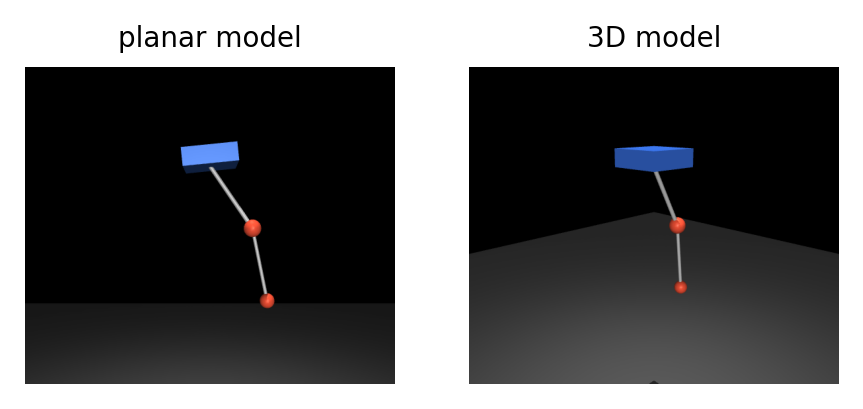
\includegraphics[width=0.55\linewidth]{figures/models.png}
  \caption{The planar and 3D MuJoCo models. Each link is a rigid rod ending in a point
  mass. Both joints are hinges about the drone's body $x$-axis, as on the hardware,
  which uses bearings rather than ball joints.}
  \label{fig:models}
\end{figure}

\paragraph{Physical model.} Both models (Fig.~\ref{fig:models}) have identical
parameters, listed in Table~\ref{tab:params}. A 1.0\,kg box-shaped drone carries two
0.5\,m links, attached 6\,cm below the drone's centre. Each link is a rod with a
sphere at its end, giving 0.15\,kg and 0.10\,kg per link and a total mass of
1.25\,kg. Each joint has viscous damping of 0.02\,N\,m\,s/rad. Matching the
hardware, both joints are \emph{single-axis hinges about the body $x$-axis}, so the
payload swings in the body $y$-$z$ plane and is rigidly attached in pitch.

\paragraph{Planar model.} The drone translates in the world $y$-$z$ plane and rolls
about $x$. The state is
$x = [y, z, \theta, q_1, q_2, \dot y, \dot z, \dot\theta, \dot q_1, \dot q_2] \in \R^{10}$,
where $q_1, q_2$ are relative joint angles. The absolute link angles are
$\phi_1 = \theta + q_1$ and $\phi_2 = \phi_1 + q_2$. The 3D model uses a free joint
for the drone, with the same two hinges.

\paragraph{Actuation.} Both models use the action interface from our proposal and from
\citet{kim2025roverfly}: normalized collective thrust and body rates,
$a = [a_T, a_\omega] \in [-1,1]^{1+n_\omega}$, with $n_\omega = 1$ in the planar model
and $3$ in 3D. Thrust is $T = \tfrac12 T_{\max}(a_T + 1)$ with
$T_{\max} = 2 m_{\text{tot}} g$, so $a = 0$ is hover thrust. A proportional inner rate
loop, standing in for the flight controller, applies body torque
$\tau = k_r(\omega_{\max} a_\omega - \omega)$, with $k_r = 0.1$\,N\,m\,s/rad and
$\omega_{\max} = 5$\,rad/s. Physics runs at 500\,Hz. Policies act at 100\,Hz in the
planar model and 50\,Hz in 3D.

\begin{table}[t]
  \centering
  \small
  \caption{Model parameters. The effective inertia is the drone's rotational block of
  the joint-space mass matrix at hover, after eliminating all other degrees of freedom
  (Schur complement).}
  \label{tab:params}
  \begin{tabular}{lll}
    \toprule
    Quantity & Value & Note \\
    \midrule
    Drone mass / total mass & 1.0\,kg / 1.25\,kg & box $0.36\times0.36\times0.12$\,m \\
    Link 1 / link 2 & 0.15 / 0.10\,kg, 0.5\,m each & rod + end mass \\
    Bare-drone inertia (roll, pitch, yaw) & 0.012, 0.012, 0.022\,kg\,m$^2$ & \\
    Effective inertia with payload & 0.012, \textbf{0.132}, 0.022\,kg\,m$^2$ & payload rigid in pitch \\
    Inner rate loop & $k_r = 0.1$\,N\,m\,s/rad, $\omega_{\max} = 5$\,rad/s & all axes \\
    \bottomrule
  \end{tabular}
\end{table}

\paragraph{Consequence of single-axis hinges.} Table~\ref{tab:params} shows that the
effective roll inertia equals the bare drone's, because the payload swings freely
about the hinge. In pitch, the drone must rotate the whole rigid payload, which
raises its effective inertia by a factor of 11. With the same rate-loop gain on every
axis, the pitch rate therefore responds with a time constant of
$J_{yy}/k_r \approx 1.3$\,s, compared with 0.12\,s in roll. Section~\ref{sec:control}
shows how we account for this, and Section~\ref{sec:exp_aware} shows what happens
when a controller does not.

%===============================================================================
\section{Classical Controllers}
\label{sec:control}

\subsection{LQR (planar)}
We linearize one control step of the simulator about hover, $x_{k+1} \approx A x_k +
B u_k$, using central finite differences through MuJoCo. This includes the inner rate
loop and the zero-order hold over five physics steps. MuJoCo's own finite-difference
routine does not apply, because the actions enter as external forces rather than as
actuators. The pair $(A, B)$ is controllable: the full controllability matrix
$[B, AB, \dots, A^{9}B]$ has rank 10. Thrust reaches only the two vertical states,
so the roll-rate input alone must span the remaining eight.

We choose the weights with Bryson's rule~\citep{bryson1975applied}, applied to the
\emph{absolute} link angles. With $x = T^{-1}\tilde x$, where
$\tilde x = [y, z, \theta, \phi_1, \phi_2, \dots]$, we use
$Q = T^\top \operatorname{diag}(1/\bar{\tilde x}_i^{\,2})\,T$ with maximum acceptable
deviations of 0.2\,m in position, 0.3\,rad in roll, 0.15\,rad in each link angle,
1\,m/s in velocity and 2\,rad/s in angular rates, and $R = 10\,I$. Penalizing absolute
rather than relative link angles roughly halved the settling time in our tuning sweep.
The larger $R$ keeps the actions away from saturation without slowing recovery, since
the slowest closed-loop mode (drone lateral motion, about $-1.26 \pm 1.79j$\,rad/s)
barely moved as $R$ varied by $100\times$.

\subsection{Flatness-based trajectory tracking}
We use the differential-flatness cascade of \citet{mellinger2011minimum} and
\citet{lee2010geometric} at the body-rate level. A reference trajectory supplies
position, velocity, acceleration and jerk ($p_r, v_r, a_r, j_r$). The controller
computes
\begin{align}
  \bfF &= m\,(a_r - K_p e_p - K_d e_v + K_i \textstyle\int e_p + g\,e_3), &
  T &= \bfF \cdot b_3, &
  b_{3,d} &= \bfF/\|\bfF\|,
\end{align}
with the desired heading completing the desired attitude $R_d$ in 3D. The rate
command is a feedforward term from the jerk plus attitude feedback. In the planar
model, $\theta_d = \operatorname{atan2}(-F_y, F_z)$ and
$\omega_d = (F_y\dot F_z - F_z\dot F_y)/\|\bfF\|^2 + k_\theta(\theta_d - \theta)$, with
$\dot\bfF = m\,j_r$. In 3D,
$\omega_d = R^\top R_d\,\omega_{\text{ff}} - k_R\,e_R$ with
$e_R = \tfrac12(R_d^\top R - R^\top R_d)^\vee$, where $\omega_{\text{ff}}$ comes from
the component of $j_r$ perpendicular to $b_{3,d}$~\citep{mellinger2011minimum}.

The controller uses only the drone's state and never the link angles. With a constant
(hover) reference it is the \emph{payload-unaware} baseline from our proposal, and its
output can later be added to a residual RL policy for trajectory following. The gains
are $K_p = \operatorname{diag}(4,4,6)$, $K_d = \operatorname{diag}(3,3,4)$, attitude
gains $(6, 6, 3)$, a $35^\circ$ tilt limit, and $K_i = 0$ unless stated otherwise.

\paragraph{Inertia-aware rate commands (3D).} Because of the pitch-inertia asymmetry
(Section~\ref{sec:system}), sending $\omega_d$ directly to the 3D model is unstable.
Instead, the controller requests the torque that would give a rate response of
bandwidth $k_\omega = 15$\,s$^{-1}$ for the real effective inertia, then inverts the
proportional rate loop:
\begin{equation}
  \tau = J_{\text{eff}}\,k_\omega(\omega_d - \omega) + \omega\times J_{\text{eff}}\,\omega,
  \qquad
  \omega_{\text{cmd}} = \omega + \tau / k_r .
\end{equation}
$J_{\text{eff}}$ is computed automatically from the MuJoCo mass matrix, so it follows
the model if the hinge axis or masses change. On hardware, the flight controller's
rate loop replaces the proportional loop modelled here. This term must then be
re-identified, or removed if that loop already tracks rates well with the payload
attached.

%===============================================================================
\section{Reinforcement Learning Setup (planar hover)}
\label{sec:rl}
The first RL task is planar hover stabilization (\texttt{HoverEnv}). Each episode
starts with the drone within $\pm5$\,cm of the target, roll within $\pm5^\circ$, links
within $\pm10^\circ$ and link rates within $\pm0.2$\,rad/s. The observation is the
13-dimensional vector
$[e_y, e_z, \sin\theta, \cos\theta, \sin q_{1,2}, \cos q_{1,2}, \dot y, \dot z,
\dot\theta, \dot q_{1,2}]$. The reward is a bounded shaped bonus minus an action
penalty,
\begin{equation}
  r = \exp\Big(-\textstyle\sum_i w_i c_i\Big) - 0.005\,\overline{a^2},
\end{equation}
where the costs $c_i$ cover position (scale 0.25\,m), roll
($1-\cos\theta$, normalized at $15^\circ$), absolute link angles (normalized at
$20^\circ$), velocity and angular rates, with weights $(1, 0.5, 0.5, 0.1, 0.1)$.
Episodes terminate if the position error exceeds 1\,m, roll exceeds $45^\circ$, or a
link angle exceeds $60^\circ$. We train PPO from Stable-Baselines3~\citep{raffin2021sb3}
with default hyperparameters, observation normalization and 8 parallel environments
for $10^6$ steps.

\todo{PPO hover results: learning curve, success rate, settling time and residual
swing after 1--8\,N pushes, using the same protocol as Table~\ref{tab:push}.}

%===============================================================================
\section{Experiments}
\label{sec:experiments}

\subsection{Disturbance recovery (planar)}
\label{sec:exp_push}
Starting from rest at hover, we push the lower mass sideways with a force $F$ for
0.1\,s at $t = 1$\,s, and simulate 10\,s. A run counts as settled once both absolute
link angles stay within $2^\circ$ and the drone stays within 5\,cm of the target until
the end of the run. We also report the largest link angle in the final 2\,s
(residual swing). The open-loop baseline holds hover thrust with zero rate command.

\begin{table}[t]
  \centering
  \small
  \caption{Planar push recovery (0.1\,s push on the lower mass). ``--'' means not
  settled within the 10\,s episode. Open loop drifts more than 2\,m from the target
  at every push magnitude.}
  \label{tab:push}
  \begin{tabular}{c|ccc|ccc}
    \toprule
    & \multicolumn{3}{c|}{LQR} & \multicolumn{3}{c}{Payload-unaware tracking (hover)} \\
    Push [N] & settle [s] & max drift [cm] & resid.\ swing [$^\circ$]
             & settle [s] & max drift [cm] & resid.\ swing [$^\circ$] \\
    \midrule
    1 & 1.41 & 11.2 & 0.0 & -- & 1.2 & 13.5 \\
    2 & 1.92 & 22.9 & 0.0 & -- & 2.5 & 26.9 \\
    3 & 2.50 & 35.4 & 0.0 & -- & 4.2 & 40.2 \\
    4 & 2.90 & 49.1 & 0.0 & -- & 6.1 & 53.2 \\
    6 & 3.23 & 79.7 & 0.0 & -- & 10.5 & 74.4 \\
    8 & 3.75 & 118.0 & 0.0 & -- & 16.8 & 84.1 \\
    \bottomrule
  \end{tabular}
\end{table}

\begin{figure}[t]
  \centering
  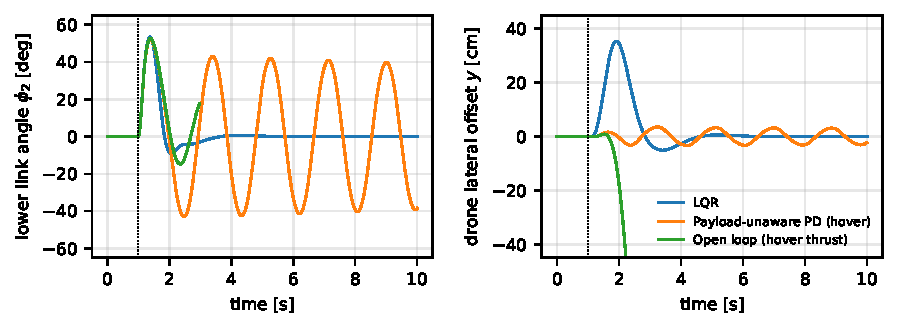
\includegraphics[width=\linewidth]{figures/push_recovery.pdf}
  \caption{Response to a 3\,N push at $t=1$\,s (dotted line). Left: lower-link angle.
  Right: drone lateral offset. LQR uses the drone's motion to damp the swing within
  2.5\,s. The payload-unaware controller keeps the drone within 4\,cm but leaves the
  payload swinging at about $40^\circ$. Open loop drifts away.}
  \label{fig:push}
\end{figure}

Table~\ref{tab:push} and Fig.~\ref{fig:push} show the trade-off the learned policy
must improve on. LQR damps the swing completely in 1.4--3.8\,s, but only by moving
the drone a long way: up to 1.2\,m for an 8\,N push, at which point the links swing
through $157^\circ$, far outside the region where its linearization is valid. The
payload-unaware controller does the opposite: it holds the drone within 17\,cm but does
nothing to damp the payload, which keeps swinging at nearly its initial amplitude.
Without control, the drone drifts more than 2\,m within about 2\,s of the push in every
case, because a zero
rate command does not hold attitude against the payload's reaction torque.
Starting from rest with the drone level, LQR also recovers from initial upper-link
angles up to $160^\circ$, tested in $10^\circ$ steps.

\subsection{Trajectory tracking}
\label{sec:exp_track}
We track three references, each starting at rest with a 2\,s speed ramp:
\begin{itemize}
  \item a circle of 0.5\,m radius at 5\,s per lap;
  \item a $1.0\times0.5$\,m figure-eight at 5\,s per lap;
  \item minimum-jerk waypoint legs of 2\,s each.
\end{itemize}
Planar references lie in the $y$-$z$ plane and 3D references in the horizontal
$x$-$y$ plane. Table~\ref{tab:track} reports the RMS error after the 3\,s warm-up and
the maximum error over each 12\,s run.

\begin{table}[t]
  \centering
  \small
  \caption{Tracking error, RMS / max in cm, and maximum link swing. ``Fails at
  $t$'' means the 3D environment's tilt or position safety limit ended the episode.}
  \label{tab:track}
  \begin{tabular}{ll|ccc}
    \toprule
    Model & Controller & Circle & Figure-8 & Waypoints \\
    \midrule
    \multirow{3}{*}{Planar} & full & 0.59 / 1.18 & 1.05 / 2.28 & 0.91 / 2.17 \\
      & no feedforward & 15.8 / 20.0 & 16.5 / 21.8 & 5.89 / 14.0 \\
      & max link swing (full) & $12.6^\circ$ & $18.4^\circ$ & $22.2^\circ$ \\
    \midrule
    \multirow{4}{*}{3D} & full & 0.27 / 0.69 & 1.27 / 2.29 & 0.74 / 1.94 \\
      & no feedforward & 19.4 / 20.6 & 27.1 / 37.1 & 8.58 / 20.2 \\
      & no inertia-aware rate cmd. & fails at 4.8\,s & fails at 4.1\,s & fails at 3.7\,s \\
      & max link swing (full) & $10.9^\circ$ & $35.1^\circ$ & $14.6^\circ$ \\
    \bottomrule
  \end{tabular}
\end{table}

\begin{figure}[t]
  \centering
  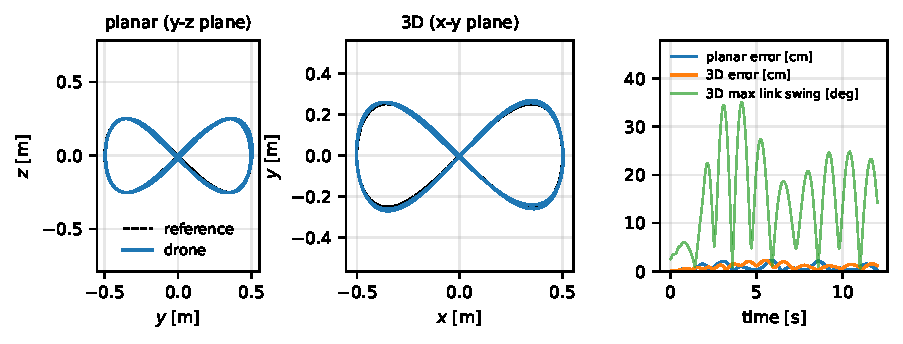
\includegraphics[width=\linewidth]{figures/tracking_figure8.pdf}
  \caption{Figure-eight tracking. Left and centre: reference (dashed) and drone path
  for the planar and 3D models. Right: tracking error and the 3D model's maximum
  link swing.}
  \label{fig:track}
\end{figure}

With feedforward, both controllers track to about 1\,cm RMS
(Fig.~\ref{fig:track}). Removing the acceleration and jerk feedforward increases the
RMS error 6--70$\times$. In 3D, removing the inertia-aware rate commands makes the drone
tip over within 5\,s on every trajectory. The links still swing by up to $35^\circ$
on the 3D figure-eight, because the controller ignores the payload. This residual
swing is exactly what an RL policy, or a residual policy added on top of this
controller, should remove.

\subsection{Payload-aware vs.\ a regular drone controller}
\label{sec:exp_aware}
To quantify the value of modelling the payload, we fly the same tracking controller
twice, with identical gains, the same integral action
($K_i = \operatorname{diag}(1,1,3)$) and the same start. The first run uses the total
mass and $J_{\text{eff}}$ ("payload-aware"). The second uses the bare drone's mass and
inertia, as a controller tuned without the payload would.

\begin{table}[t]
  \centering
  \small
  \caption{Payload-aware vs.\ regular (bare-drone) controller, RMS tracking error in
  cm. Both include integral action.}
  \label{tab:aware}
  \begin{tabular}{l|ccc|ccc}
    \toprule
    & \multicolumn{3}{c|}{Planar} & \multicolumn{3}{c}{3D} \\
    & Circle & Figure-8 & Waypoints & Circle & Figure-8 & Waypoints \\
    \midrule
    Payload-aware & 0.64 & 1.16 & 0.93 & 0.30 & 1.22 & 0.76 \\
    Regular & 5.40 & 5.98 & 3.47 & fails at 7.4\,s & fails at 6.7\,s & fails at 5.2\,s \\
    \bottomrule
  \end{tabular}
\end{table}

\begin{figure}[t]
  \centering
  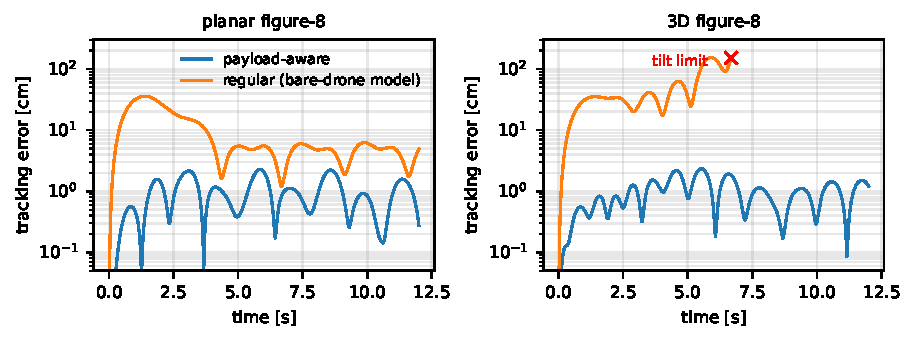
\includegraphics[width=\linewidth]{figures/aware_vs_regular.pdf}
  \caption{Tracking error on the figure-eight (log scale). The regular controller
  first sags by about 35\,cm from the underestimated mass, which the integrator slowly
  removes. In 3D it then tips past the tilt limit, because it underestimates the
  pitch inertia by a factor of 11.}
  \label{fig:aware}
\end{figure}

Table~\ref{tab:aware} and Fig.~\ref{fig:aware} separate the two effects. In the
planar model only the mass is wrong, because roll is about the hinge axis and the
payload swings freely there. The integrator recovers the height, but tracking remains
4--8$\times$ worse. In 3D the inertia mismatch is decisive: the regular controller's
pitch commands are about $11\times$ too weak, and it tips over on every moving
trajectory. For hardware, this means the flight controller needs either the total
mass or a hover-thrust estimate, and a pitch rate loop retuned with the payload
attached, before we can compare learned and classical controllers fairly.

%===============================================================================
\section{Discussion and Next Steps}
\label{sec:next}
The baselines bracket the behaviour we want from the learned policy. LQR damps the
swing but needs large drone excursions and relies on a hover linearization. The
payload-unaware controller holds the drone precisely but leaves the payload
oscillating. Our next steps are:
\begin{enumerate}
  \item \textbf{Planar RL:} finish PPO hover and push-recovery training, then compare
        with SAC and TD3 under the protocol of Table~\ref{tab:push}. Add the
        region-of-attraction and parameter-mismatch metrics from the proposal.
  \item \textbf{3D environment:} replace the placeholder reward, add the push
        disturbance schedule, and extend LQR to 3D using the same numerical
        linearization.
  \item \textbf{Robustness:} randomize payload mass, link lengths and actuation delay
        during training, and evaluate under mismatch.
  \item \textbf{Hardware:} identify the real rate loop with the payload attached,
        set the tracking controller's mass and inertia accordingly, and generate
        repeatable disturbances with a scripted manoeuvre, as proposed.
\end{enumerate}
\todo{Timeline and division of work for the remaining weeks.}

%===============================================================================
\bibliography{references}

\end{document}
